\documentclass{ceurart}
% Five-page ongoing-work version of the manuscript; see README.md for build and review status.
% No class, page-geometry or body-font overrides are applied to the CEURART build.
\usepackage{listings}
\usepackage{tabularx}
\usepackage{booktabs}
\usepackage{tikz}
\usetikzlibrary{arrows.meta,positioning}
\usepackage{xurl}
\newcommand{\term}[1]{\texttt{#1}}
\lstset{basicstyle=\small\ttfamily,breaklines=true,columns=fullflexible,
  keepspaces=true,showstringspaces=false,frame=single,
  aboveskip=6pt,belowskip=6pt}
\emergencystretch=1em
\begin{document}

\copyrightyear{2027}
\copyrightclause{Copyright for this paper by its authors.
  Use permitted under Creative Commons License Attribution 4.0
  International (CC BY 4.0).}
\conference{SWAT4HCLS 2027, February 1--4, 2027, Basel, Switzerland}

\title{VCF Core: A Semantic Foundation for RDF Representations of VCF}

\author[1,2]{Elias Crum}[
orcid=0009-0005-3991-754X,
email=elias.crum@ugent.be
]
\cormark[1]
\author[2]{Bart Buelens}[
orcid=0000-0001-7734-3747,
email=bart.buelens@vito.be
]
\author[2]{Gökhan Ertaylan}[
orcid=0000-0001-5602-6435,
email=gokhan.ertaylan@vito.be
]
\author[1]{Ruben Taelman}[
orcid=0000-0001-5118-256X,
email=ruben.taelman@ugent.be
]
\address[1]{IDLab, Department of Electronics and Information Systems, Ghent University -- imec, Belgium}
\address[2]{Flemish institute for Technological Research (VITO) Mol, Belgium}
\cortext[1]{Corresponding author.}



% Short-paper revision: retain the source manuscript's claims and terminology.
% The ongoing-work framing concerns assessment, refinement and application,
% not whether the existing vocabulary and release artifacts are available.
\begin{abstract}
Medical applications of genomic data depend on connecting variant observations to clinical information and biomedical knowledge.
Linked Data offers a framework for this integration, but the Variant Call Format (VCF) does not natively provide an RDF representation of the observations and their interpretation context.
We present ongoing work on VCF Core, a shared semantic target for representing VCF files, header declarations, records, annotations and sample data.
The current vocabulary integrates existing provenance and genomic models while retaining VCF-specific field definitions, ordering and missingness.
Expanded sample calls and condensed, sample-ordered vectors support different representation needs, with version-specific artifacts addressing VCF 4.1--4.5.
Initial assessments provide evidence of broad representation coverage, while validation and cross-version review remain ongoing.
We outline how this foundation could support reusable conversion engines and traceable biomedical queries, and invite contributions to its mappings, assessment and application.
\end{abstract}
\begin{keywords}
Variant Call Format\sep RDF\sep Genomic data\sep Vocabulary\sep Data integration\sep SHACL
\end{keywords}
\maketitle

\section{Introduction}

Genomic data are increasingly useful in medicine when integrated with other patient, public, and/or proprietary information.
A drug-response assessment, for example, depends on the relationship between a patient's genomic findings, a prescribed medication, and the knowledge used to interpret that relationship~\cite{lee2022cpic}.
The presence of a variant alone does not establish these connections.
Semantic approaches provide a basis for making them explicit: HERO-Genomics addresses integration of genomic and biomedical information, while Semantic Beacons demonstrates federated queries over variant data and public knowledge graphs~\cite{cazzaro2025hero,bodrug2025semantic}.
These investigations motivate a reusable representation of the source observations on which interpretation depends.

The Variant Call Format (VCF) is widely used to exchange genomic variant data~\cite{danecek2011vcf}.
It already supports database identifiers, reference information and extensible annotations, so its limitation is not that data linking is impossible.
Rather, VCF does not natively expose these elements and their relationships as RDF.
A value often depends on a header declaration, an ordered allele list, or the structure of a sample column for its interpretation~\cite{vcf45}.
Converting only selected variant attributes can leave those dependencies implicit.

Existing approaches, including the Genomic Feature and Variation Ontology (GFVO) and VCF2RDF, provide important foundations~\cite{baran2015gfvo,penha2017vcf2rdf}.
The next step is therefore not to establish that VCF can be represented in RDF, but to provide a shared, version-aware target that combines broad source-format coverage with explicit connections to existing models.
Here, we present VCF Core Vocabulary 2.1.0~\cite{vcfc210}, developed from our earlier VCF-RDFizer Vocabulary~\cite{crum2025semantifying}.
The vocabulary and supporting artifacts are available; ongoing work concerns establishing their semantic fidelity across VCF versions, refining validation, and evaluating reuse.
Throughout, \term{vcfc:} denotes \url{https://w3id.org/vcf-core/vocab#}.

\section{VCF as a semantic representation problem}
\label{sec:vcf}

A VCF file contains meta-information lines, a column-header line and data records.
The header identifies the format version and can describe reference sequences and the fields used in records.
Each record describes a genomic position, a reference allele and one or more ordered alternative alleles, together with quality, filter and annotation information.
INFO fields describe the record, whereas FORMAT keys describe the contents of sample columns~\cite{vcf45}.

For example, a record with reference allele A, alternative allele G and \term{FORMAT=GT:DP} may contain the sample value \term{0/1:42}.
Here, the genotype refers to one reference and one alternative allele, and 42 is the read depth.
The value \term{./.:.} instead indicates missing genotype and depth values.
Genotype indices depend on the allele list, while the meaning of each sample value depends on its FORMAT key.
Likewise, a header's \term{Number=A} means one value per alternative allele, whereas \term{Number=R} also includes the reference allele~\cite{vcf45}.
Representing VCF therefore requires more than assigning predicates to columns.

VCF 4.1--4.5 share these basic structures but differ in supported declarations and constraints~\cite{htsspecs,vcf45}.
For example, the CIPOS field describes uncertainty around a reported position.
Its declared cardinality changes from two values in VCF 4.1--4.3 to two per alternative allele in 4.4--4.5.
A common model should retain the declared version rather than interpreting historical data under newer rules.
It should also distinguish source observations from biological interpretation: two files may describe the same alteration with different quality scores, and a sample column is not necessarily a patient.

\section{The VCF Core vocabulary}
\label{sec:design}

VCF Core separates a \term{VCFFile}, its \term{VCFHeader}, individual \term{VCFRecord} resources and a \term{VariantCall} associated with each record.
The call groups quality, filter, annotation and genotype information; it is a modeling abstraction rather than an additional source line.
Figure~\ref{fig:model} summarizes this structure and the two sample representations.

The file specializes \term{dcat:Distribution} and \term{prov:Entity}, while records and calls provide further attachment points for provenance~\cite{prov2013,vcfc210}.
Source-based identifiers keep observations from different files distinct.
The property \term{asSequenceAlteration} connects a record or call to a separately described Sequence Ontology (SO) alteration, while FALDO supplies location and reference descriptions~\cite{eilbeck2005so,bolleman2016faldo}.
VCF Core therefore preserves source context without introducing a competing general-purpose model of biological variation or location.

% The original model diagram is retained as a compact alternative to the
% detailed term-by-term account in the longer manuscript.
\begin{figure}[htbp]
\centering
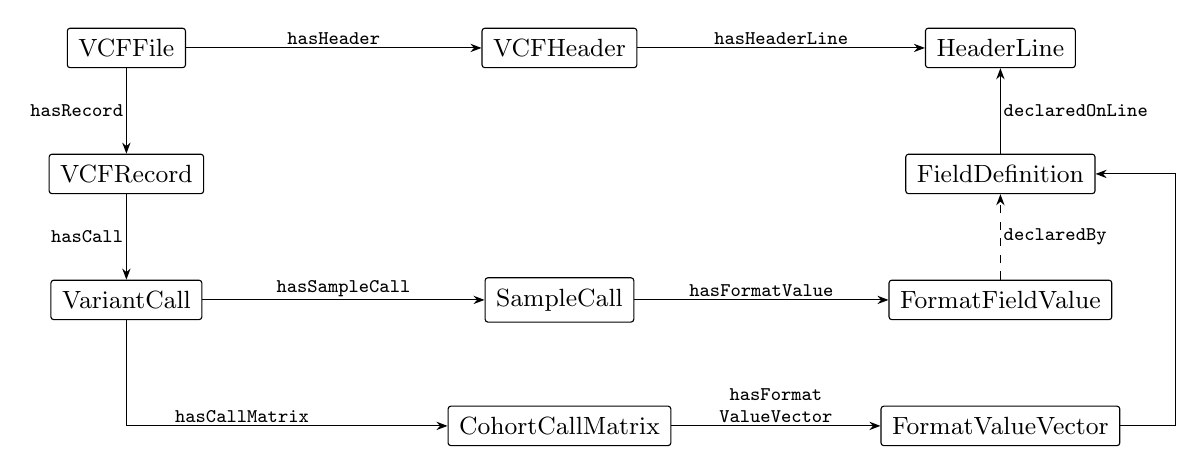
\begin{tikzpicture}[x=1mm,y=1mm,
  box/.style={draw,rounded corners=1pt,align=center,font=\small,inner sep=4pt},
  edge/.style={-{Stealth[length=4pt]},thin},
  lab/.style={font=\scriptsize\ttfamily,fill=white,inner sep=1pt,align=center}]
\node[box] (file) at (17,0) {VCFFile};
\node[box] (header) at (72,0) {VCFHeader};
\node[box] (line) at (128,0) {HeaderLine};
\node[box] (record) at (17,-16) {VCFRecord};
\node[box] (call) at (17,-32) {VariantCall};
\node[box] (definition) at (128,-16) {FieldDefinition};
\node[box] (sample) at (72,-32) {SampleCall};
\node[box] (value) at (128,-32) {FormatFieldValue};
\node[box] (matrix) at (72,-48) {CohortCallMatrix};
\node[box] (vector) at (128,-48) {FormatValueVector};
\draw[edge] (file) -- node[lab,above] {hasHeader} (header);
\draw[edge] (header) -- node[lab,above] {hasHeaderLine} (line);
\draw[edge] (file) -- node[lab,left] {hasRecord} (record);
\draw[edge] (record) -- node[lab,left] {hasCall} (call);
\draw[edge] (definition) -- node[lab,right] {declaredOnLine} (line);
\draw[edge] (call) -- node[lab,above] {hasSampleCall} (sample);
\draw[edge] (sample) -- node[lab,above] {hasFormatValue} (value);
\draw[edge] (call.south) |- node[lab,above,pos=0.68] {hasCallMatrix} (matrix);
\draw[edge] (matrix) -- node[lab,above] {hasFormat\\ValueVector} (vector);
\draw[edge,dashed] (value) -- node[lab,right] {declaredBy} (definition);
\draw[edge] (vector.east) -- ++(7,0) |- (definition.east);
\end{tikzpicture}
\caption{Selected VCF Core relationships; prefixes are omitted. Both sample profiles retain the file, record and header context. An expanded value can link to its definition through \term{declaredBy}; the equivalent relation is required for a condensed vector. Sample identity and ordering are described through \term{VCFSample} and \term{SampleSet}.}
\label{fig:model}
\end{figure}

Header declarations are retained because they determine how values should be read.
Field definitions expose identifiers, types, cardinalities and descriptions, while separate header-line resources describe their occurrence in a file.
Values can link to their defining declaration through \term{declaredBy}.
Lexical values preserve source tokens, including missingness and genotype separators; optional parsed properties support suitable scalar queries.
Ordered allele resources retain the context needed to interpret genotype indices and allele-dependent annotations~\cite{vcfc210}.

The expanded profile exposes per-sample \term{SampleCall} and \term{FormatFieldValue} resources for direct graph queries and annotation.
The condensed profile instead groups sample-ordered vectors by FORMAT key through a \term{CohortCallMatrix} and a shared \term{SampleSet}.
Its initial text encoding retains individual sample values, including missing values, rather than replacing them with cohort summaries.
Condensed cells require decoding before per-sample comparisons; they are not directly bound by ordinary basic graph patterns.
The profiles offer different graph granularities, but their relative storage and query performance still require evaluation.

\section{Building on existing semantic models}
\label{sec:alignments}

The usefulness of VCF Core depends on its relationship to models already used for genomic data.
GFVO explicitly addressed VCF 4.1 and 4.2, and VCF2RDF demonstrated source-preserving semantic conversion~\cite{baran2015gfvo,penha2017vcf2rdf}.
HERO-Genomics includes files and records within a broader integration model, while the Genome Variation Ontology (GVO) addresses detailed variation descriptions~\cite{cazzaro2025hero,kawashima2023gvo}.
The GA4GH Variation Representation Specification (VRS) provides computable variation descriptions and federated identification, rather than a representation of every source-file detail~\cite{wagner2021vrs}.
These are complementary purposes, not successive attempts at the same task.

VCF Core brings a format-oriented representation, explicit VCF 4.1--4.5 artifacts, alternative sample profiles and inspectable alignments into one maintained target.
Extending the documented scope while retaining historical declarations builds on earlier work; it is not a head-to-head coverage ranking.
The earlier projects have not been assessed under a common rubric here.

Direct reuse and cross-model alignment are kept distinct.
PROV, DCAT, SO and FALDO contribute to the core representation, while 123 curated mappings document connections to variation models and reference ontologies~\cite{vcfc210}.
The mappings are maintained in the Simple Standard for Sharing Ontological Mappings (SSSOM), with an RDF bridge for reuse~\cite{matentzoglu2022sssom}.
They record correspondences with different strengths, not unrestricted OWL equivalence or the instance links needed for a biomedical query.
Reviewing these correspondences with the relevant communities remains an important part of the work.

\section{Specification coverage and ongoing assessment}
\label{sec:coverage}

VCF Core uses a shared model with version-specific registries and validation overlays for VCF 4.1--4.5~\cite{vcfc210}.
The VCF 4.5 registry includes 122 reserved INFO and FORMAT declarations.
Validation combines portable SHACL structure checks, SPARQL-based cross-resource checks and raw/parsed-value consistency checks~\cite{shacl2017,vcfc210}.
Version-specific rules are applied according to the owning file's declared format.

An initial developer-curated VCF 4.5 assessment records preserved, structured representations for all 104 inventoried logical-model constructs, with enforcement evidence for 87.
This supports broad representation coverage under that rubric, not complete conformance.
A complementary assessment derived from VCF 4.1--4.5 specifications exposes remaining validation and evidence gaps, including unresolved rule interpretations and an incomplete version-transition review~\cite{vcfc210}.
The assessments address different questions and should not be combined into a single coverage percentage.

Ongoing assessment aims to establish VCF Core as a faithful semantic representation across the supported versions through review of requirements, mappings and executable examples.
Priorities include strengthening evidence for less-tested constructs, resolving validation gaps, and checking whether recovered values and query answers preserve the source meaning.
Independent review is particularly important because the current logical-model inventory was curated by the vocabulary's developers.

The release provides OWL/Turtle modules, SHACL profiles, examples, versioned registries, SSSOM mappings and documentation~\cite{vcfc210}.
VCF-RDFizer supplies an implementation lineage, although its cited snapshot uses the predecessor namespace and is not evidence of complete VCF Core 2.1.0 support~\cite{vcfrConverter2026}.
Small fixtures and a synthetic query example provide implementation evidence, but do not establish cohort-scale performance, general converter correctness or clinical validity.


\paragraph{A bounded query example.}
Listing~\ref{lst:depth} illustrates how a representation can be assessed through recovered values and query answers.
The supplied synthetic record has three sample values: \term{0/1:42}, \term{0/0:18} and \term{./.:.}, with \term{FORMAT=GT:DP}.
On its expanded graph, the query returns SAMPLE1 with depth 42; decoding the corresponding condensed graph gives the same selection and recovers the same six FORMAT cells~\cite{vcfc210}.
The threshold is illustrative, not a clinical quality standard.
This bounded check provides a starting point for broader competency queries and source-value comparisons rather than evidence of general fidelity.

\begin{lstlisting}[caption={Direct access to sample depth in the expanded representation.},label={lst:depth}]
PREFIX vcfc: <https://w3id.org/vcf-core/vocab#>
SELECT ?sampleName ?depth WHERE {
  ?file vcfc:representationProfile vcfc:ExpandedRepresentation ;
        vcfc:hasRecord/vcfc:hasCall/vcfc:hasSampleCall ?call .
  ?call vcfc:forSample/vcfc:sampleName ?sampleName ;
        vcfc:hasFormatValue ?value .
  ?value vcfc:declaredBy/vcfc:fieldId "DP" ;
         vcfc:fieldValueInteger ?depth .
  FILTER (?depth >= 20)
}
\end{lstlisting}

\section{Discussion}
\label{sec:discussion}

VCF Core can make more of the evidence already present in a VCF file available to semantic applications.
It retains observations and their interpretation context, while other models describe specimens, patients, diseases, treatments and biological variation.
For example, two laboratories could link records to a common variation description after reference-aware normalization, while retaining distinct quality values and provenance.
A disease-association assertion could then be connected to that description without being copied into each source record.
The vocabulary provides connection points; normalization and instance mappings still need to be implemented and evaluated.

A shared target could also separate conversion strategy from representation decisions.
A hospital inspecting individual calls may choose expanded values, while a research group handling a cohort may choose condensed vectors and decode selected fields when needed.
Both can retain the same file, header and record model.
A pipeline processing historical VCF 4.2 and newer VCF 4.5 data could select the appropriate registry and validation overlay rather than imposing one version's rules on all files.
Comparisons should establish recovered-value and query-answer agreement before measuring conversion time, memory or storage.

\paragraph{Medically relevant querying.}
A prospective pharmacogenomic question is: \emph{Which patients with an active clopidogrel prescription have an externally established CYP2C19 phenotype relevant to their treatment indication, and which source observations support that assessment?}
A query could join prescriptions, reviewed phenotype assessments and applicable guideline knowledge to specimen-linked calls and their provenance~\cite{lee2022cpic}.
Variant processing and clinical interpretation remain separate steps; a VCF genotype token must not be treated as a metabolizer phenotype~\cite{pharmcatmethods}.

Similarly, a rare-disease query could connect candidate alterations to disease-associated genes and a patient's recorded phenotypic features, using resources such as HPO~\cite{hpo}.
An oncology query could join tumour alterations to cancer-specific therapeutic evidence from a resource such as CIViC, then retrieve matched-normal observations and source quality fields~\cite{griffith2017civic}.
A missing call would remain missing evidence, not proof of absence.
These are research scenarios requiring additional biomedical data, reviewed instance links and access controls, not evaluated clinical workflows.

\paragraph{Opportunities for contribution.}
The immediate opportunity is to investigate these uses against a common representation rather than repeatedly reconstructing VCF semantics within each application.
Contributions of version-specific examples, counterexamples to validation rules, reviewed alignments and competency queries would strengthen both the vocabulary and its assessment.
Converter and query-engine implementations could then test fidelity and practical trade-offs against the same target.
This work should establish answer correctness and provenance recovery before making claims about medical utility or query speed.

\section{Conclusion}

VCF Core provides a shared semantic foundation for VCF observations and their interpretation context, combining reuse of existing models with source structure, alternative sample representations and version-specific artifacts for VCF 4.1--4.5.
The current release provides a basis for reuse, while establishing semantic fidelity across versions and applications remains ongoing.
We invite contributions to its assessment, alignments and use cases so that this foundation can develop into a shared target for genomic data integration.

\begin{acknowledgments}
Project funding provided from the Research Foundation -- Flanders (FWO) (SB Fellowship 1S27825N).
Ruben Taelman is a postdoctoral fellow of the Research Foundation -- Flanders (FWO) (1202124N).
\end{acknowledgments}

\section*{Declaration on Generative AI}
OpenAI Codex and Claude assisted with preparatory work on the vocabulary, assessment artifacts and manuscript.
ChatGPT assisted with restructuring, prose revision, reference checks and prospective query examples, and with shortening this version.

\label{endofmain}
\clearpage
{\interlinepenalty=10000
\bibliography{sources}}
\end{document}
